\documentclass[a4paper,12pt]{article}
\usepackage[utf8]{vietnam}
\usepackage{geometry}
\usepackage{graphicx}
\usepackage{float}
% \usepackage{hyperref} % Commented out to avoid option clash with the declaration below
\usepackage{listings}
\usepackage{xcolor}
\usepackage{fancyhdr}
\usepackage{booktabs}
\usepackage{longtable}
\usepackage{array}
\usepackage{ragged2e}
\usepackage{graphicx}
\usepackage{caption}
\usepackage{enumitem}
\usepackage{amssymb} % \square for checklist boxes
\usepackage{xcolor}
% \usepackage{fvextra} % Commented out to prevent conflict with listings
\usepackage[colorlinks=true, linkcolor=blue!50!black, urlcolor=blue!50!black, citecolor=blue!50!black]{hyperref}
\usepackage{titlesec}
\usepackage{parskip}
\usepackage{float}

\sloppy
\tolerance=9999
\emergencystretch=3em
\hbadness=10000

\newcolumntype{L}[1]{>{\RaggedRight\arraybackslash}p{#1}}

\titleformat{\section}{\Large\bfseries}{\thesection}{0.6em}{}
\titleformat{\subsection}{\large\bfseries}{}{0em}{}
\titleformat{\subsubsection}{\normalsize\bfseries}{}{0em}{}

\newenvironment{noteblock}
  {\begin{quote}\itshape}
  {\end{quote}}

\newenvironment{imgplaceholder}[2]
  {\begin{figure}[H]\centering
   \fbox{\begin{minipage}{0.9\textwidth}\centering\vspace{1.2cm}
   \textit{[Chưa có ảnh — vị trí tham chiếu]}\\[0.3cm]
   \texttt{#1}
   \vspace{1.2cm}\end{minipage}}
   \caption{#2}}
  {\end{figure}}
% Cấu hình hiển thị code
\definecolor{codegray}{rgb}{0.5,0.5,0.5}
\definecolor{codegreen}{rgb}{0,0.6,0}
\definecolor{backcolour}{rgb}{0.95,0.95,0.92}
\definecolor{codepurple}{rgb}{0.58,0,0.82}
\lstdefinestyle{mystyle}{
    backgroundcolor=\color{backcolour},   
    commentstyle=\color{codegreen},
    keywordstyle=\color{magenta},
    numberstyle=\tiny\color{codegray},
    stringstyle=\color{codepurple},
    basicstyle=\ttfamily\footnotesize,
    breakatwhitespace=false,         
    breaklines=true,                 
    captionpos=b,                    
    keepspaces=true,                 
    numbers=left,                    
    numbersep=5pt,                  
    showspaces=false,                
    showstringspaces=false,
    showtabs=false,                  
    tabsize=2
}
\lstset{style=mystyle}

% Cấu hình trang
\geometry{left=2.5cm, right=2.5cm, top=2cm, bottom=2cm}
\pagestyle{fancy}
\fancyhf{}
\rhead{Báo cáo Linux Capstone }
\lhead{Môn học: Hệ điều hành Linux \& Ứng dụng}
\cfoot{\thepage}

\begin{document}

% ----------------------------------------------------------------
% TRANG BÌA
% ----------------------------------------------------------------
\begin{titlepage}
    \begin{center}
        \vspace*{1cm}
        \Large\textbf{TRƯỜNG ĐẠI HỌC KHOA HỌC TỰ NHIÊN}\\
        \large\textbf{ĐẠI HỌC QUỐC GIA TP. HỒ CHÍ MINH}\\
        \vspace{1.5cm}
        
        \begin{figure}[H]
            \centering
            \fbox{\begin{minipage}{0.35\textwidth}\centering\vspace{1.5cm}
            \textit{[Trường ĐHKHTN — Logo Placeholder]}\vspace{1.5cm}\end{minipage}}
        \end{figure}
        \vspace{1.5cm}
        
        \LARGE\textbf{Linux Capstone}\\
        \vspace{0.3cm}
        \Large\textbf{Hệ điều hành Linux \& Ứng dụng}\\
        \vspace{2cm}
        
        \begin{tabular}{lll}
            \textbf{Sinh viên thực hiện:} & Nguyễn Lê Nhật Duy & 23127180 \\
                                         & Lê Nguyễn Nhật Khánh & 23127206 \\
                                         & Lê Hoàng Long & 23127412 \\
                                         & Nguyễn Văn Bảo Phúc & 23127457 \\
                                         & Cao Lê Gia Phú & 23127535 \\
        \end{tabular}
        
        \vfill
        \large TP. HỒ CHÍ MINH, NĂM 2026
    \end{center}
\end{titlepage}





% ===================== LAYOUT & UTILITIES =====================


\subsection*{Thành viên và phân công}


\begin{center}
\begin{tabular}{@{}cL{4.5cm}L{5.5cm}L{3cm}@{}}
\toprule
\textbf{STT} & \textbf{Họ và tên} & \textbf{Phân công thực tế} & \textbf{Mức đóng góp} \\
\midrule
1 & Cao Lê Gia Phú & hạ tầng và mạng  & 100\% \\
2 &  Nguyễn Văn Bảo Phúc & reverse proxy và bảo mật web   & 100\% \\
3 & Nguyễn Lê Nhật	Duy & ứng dụng và systemd  & 100\% \\
4 &  Lê Nguyễn Nhật Khánh &CSDL và sao lưu  & 100\% \\
5 &  Lê Hoàng Long & bộ công cụ tự động hóa và cảnh báo  & 100\% \\

\bottomrule
\end{tabular}
\end{center}
\vspace{1.5cm}

\hrule

\vspace{0.5cm}
\newpage
% ----------------------------------------------------------------
% MỤC LỤC
% ----------------------------------------------------------------
\tableofcontents
\newpage
% ----------------------------------------------------------------
% NỘI DUNG BÁO CÁO
% ----------------------------------------------------------------

\section{Tổng quan hệ thống}
\subsection{Hướng đồ án đã chọn}
Dự án Capstone triển khai hệ thống bao gồm một ứng dụng Web Backend (FastAPI), cơ sở dữ liệu MySQL, và Nginx làm Web Server kiêm Reverse Proxy. Toàn bộ kiến trúc được triển khai trên nền tảng ảo hóa Proxmox Virtual Environment (PVE) và hệ điều hành Ubuntu 22.04 LTS Server.

\subsection{Sơ đồ mạng và các máy ảo (VM)}
Hệ thống được thiết kế theo mô hình phân vùng mạng an toàn, cô lập máy dịch vụ chính và máy sao lưu khỏi internet bên ngoài bằng cách sử dụng cổng trung chuyển (Jump Host / Bastion Host):
\begin{enumerate}
    \item \textbf{Mạng ngoài (External/WAN - Bridge \texttt{vmbr0})}: Liên kết trực tiếp card vật lý trên máy chủ Proxmox, cung cấp IP mạng ngoài cho máy ảo \texttt{jump-host} để quản trị viên có thể kết nối từ xa.
    \item \textbf{Mạng LAN nội bộ (Private LAN - Bridge \texttt{vmbrcs})}: Switch ảo cô lập hoàn toàn (không gán cổng mạng vật lý). Sử dụng dải IP nội bộ \texttt{10.10.10.0/24} với Gateway ảo trên Host PVE là \texttt{10.10.10.1}.
\end{enumerate}

Sơ đồ kết nối hệ thống được mô tả ở hình dưới đây:
\begin{figure}[H]
    \centering
    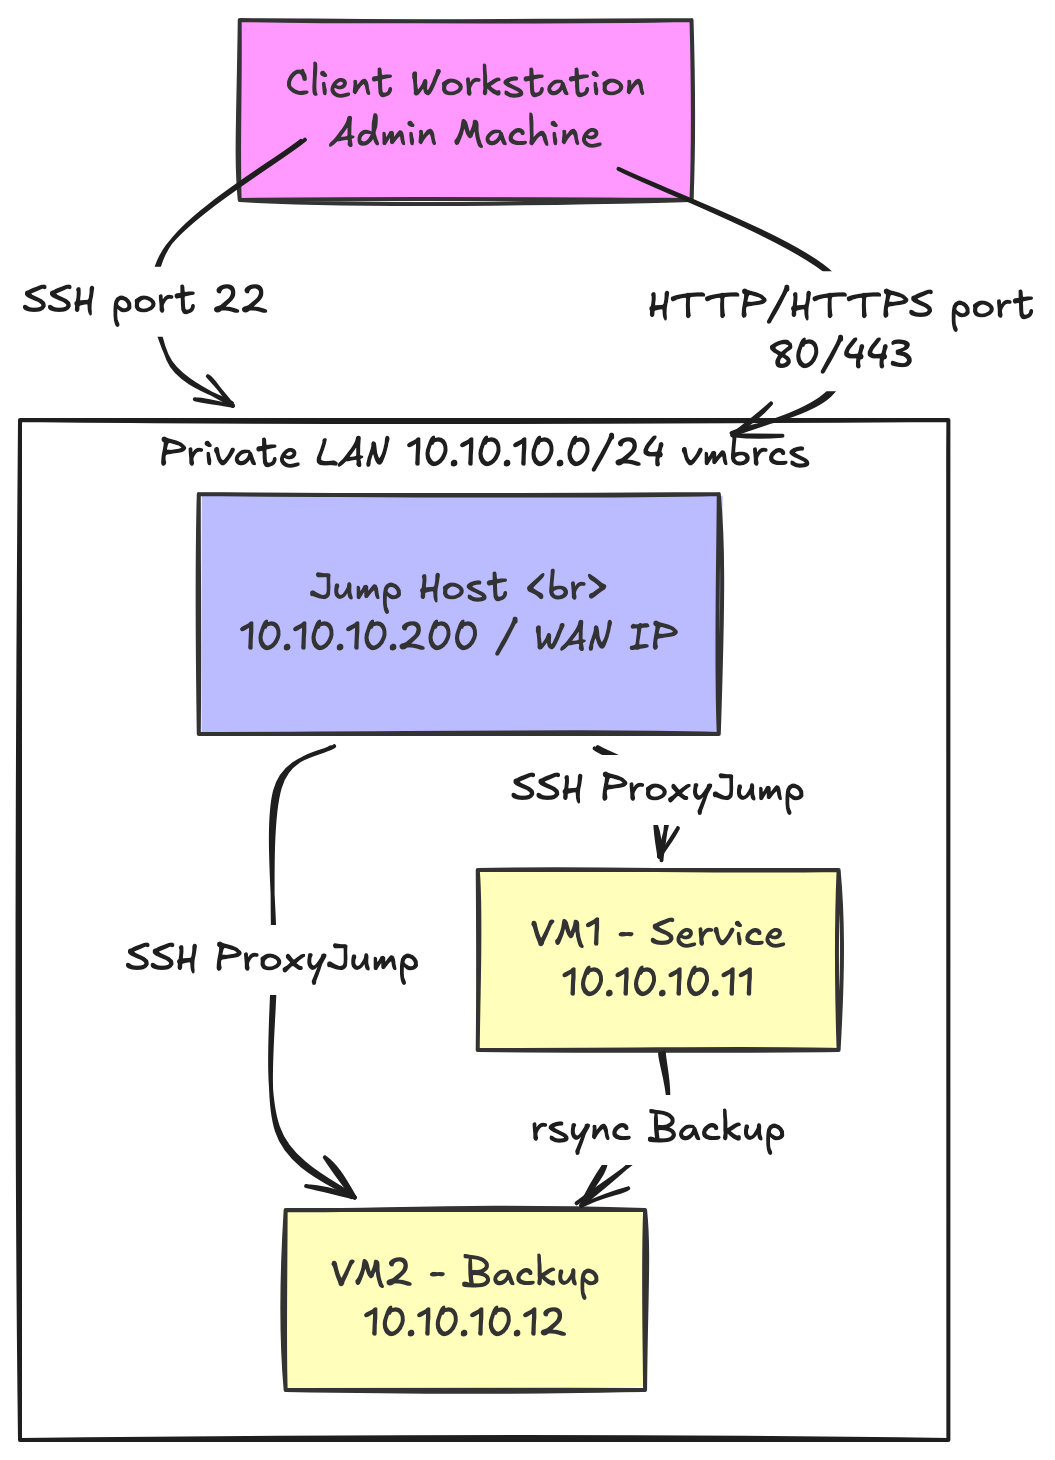
\includegraphics[width=0.85\textwidth]{images/so_do.png}
    \caption{Sơ đồ kiến trúc kết nối mạng an toàn của hệ thống}
\end{figure}

Danh sách các máy ảo được cấu hình và vận hành đồng thời trên node Proxmox:
\begin{longtable}{|c|L{2.5cm}|c|c|L{3cm}|L{3.5cm}|}
\hline
\textbf{ID VM} & \textbf{Hostname} & \textbf{vCPU} & \textbf{RAM} & \textbf{Dải IP kết nối} & \textbf{Vai trò hệ thống} \\ \hline
200 & \texttt{jump-host} & 1 & 1.00 GiB & WAN (Bridge \texttt{vmbr0}) \newline \texttt{10.10.10.200} (\texttt{vmbrcs}) & Cổng SSH Jump Host (Bastion) trung chuyển \\ \hline
203 & \texttt{vm1-svc} & 2 & 2.00 GiB & \texttt{10.10.10.11} (\texttt{vmbrcs}) & Máy chủ dịch vụ chính (Nginx, App, MySQL) \\ \hline
202 & \texttt{vm2-backup} & 2 & 2.00 GiB & \texttt{10.10.10.12} (\texttt{vmbrcs}) & Máy chủ nhận và lưu trữ bản sao lưu \\ \hline
\end{longtable}

\subsection{Cấu hình lưu trữ phần cứng}
\begin{itemize}
    \item \textbf{\texttt{jump-host}}: Sử dụng 1 ổ cứng ảo \texttt{scsi0} (20 GB) chứa HĐH.
    \item \textbf{\texttt{vm1-svc}}: Sử dụng 2 ổ cứng ảo:
    \begin{itemize}
        \item \texttt{scsi0} (20 GB): Chứa hệ điều hành Ubuntu Server.
        \item \texttt{scsi1} (10 GB): Định dạng ext4, mount tự động qua \texttt{/etc/fstab} vào thư mục \texttt{/mnt/data}. Đây là phân vùng độc lập lưu trữ MySQL và mã nguồn ứng dụng, giúp bảo vệ dữ liệu dự án tách biệt khỏi phân vùng HĐH.
    \end{itemize}
    \item \textbf{\texttt{vm2-backup}}: Sử dụng 2 ổ cứng ảo:
    \begin{itemize}
        \item \texttt{scsi0} (20 GB): Chứa hệ điều hành Ubuntu Server.
        \item \texttt{scsi1} (20 GB): Định dạng ext4, mount tự động qua \texttt{/etc/fstab} vào thư mục \texttt{/mnt/backup} chuyên dụng cho lưu trữ bản sao lưu và quản lý xoay vòng.
    \end{itemize}
\end{itemize}

\subsection{Giải pháp truy cập quản trị từ xa (SSH ProxyJump)}
Vì \texttt{vm1-svc} và \texttt{vm2-backup} nằm trong mạng nội bộ riêng tư \texttt{vmbrcs}, quản trị viên không thể SSH trực tiếp. Giải pháp SSH ProxyJump được thiết lập như sau:
\begin{enumerate}
    \item Đăng nhập bằng khóa SSH Ed25519 từ máy Client cá nhân. Tắt đăng nhập bằng mật khẩu (\texttt{PasswordAuthentication no}) và tài khoản root (\texttt{PermitRootLogin no}) trên tất cả các VM.
    \item Cấu hình file SSH Client trên máy quản trị (\texttt{~/.ssh/config}) để tạo kết nối trong suốt:
\begin{lstlisting}[language=bash]
Host jump
    HostName <IP_JUMP_HOST_WAN>
    User sysadmin
    IdentityFile ~/.ssh/id_ed25519

Host vm1-svc
    HostName 10.10.10.11
    User sysadmin
    ProxyJump jump
    IdentityFile ~/.ssh/id_ed25519

Host vm2-backup
    HostName 10.10.10.12
    User sysadmin
    ProxyJump jump
    IdentityFile ~/.ssh/id_ed25519
\end{lstlisting}
    \item Lệnh để SSH trực tiếp vào máy chủ dịch vụ thông qua Jump Host:
    \begin{lstlisting}[language=bash]
ssh vm1-svc
    \end{lstlisting}
\end{enumerate}

\newpage
\section{Các bước xây dựng hệ thống}

\subsection{Cài đặt các gói phần mềm cần thiết}
Trên máy chủ dịch vụ \texttt{vm1-svc}, thực hiện cài đặt các công cụ và dịch vụ cốt lõi:
\begin{lstlisting}[language=bash]
sudo apt update
sudo apt install -y nginx ufw fail2ban auditd audispd-plugins lynis openssl curl sshpass
\end{lstlisting}

\subsection{Khởi tạo tài khoản quản trị viên}
Khởi tạo các tài khoản có quyền quản trị qua \texttt{sudo} thay cho tài khoản \texttt{root}:
\begin{lstlisting}[language=bash]
# Tao user sysadmin va dat mat khau
useradd -m -s /bin/bash sysadmin
passwd sysadmin
usermod -aG sudo sysadmin

# Tao user devops va dat mat khau
useradd -m -s /bin/bash devops
passwd devops
usermod -aG sudo devops
\end{lstlisting}

Import Public Key từ máy Client quản trị vào tệp \texttt{authorized\_keys} của các user trên \texttt{vm1-svc}:
\begin{lstlisting}[language=bash]
# Cho sysadmin
mkdir -p /home/sysadmin/.ssh
cat >> /home/sysadmin/.ssh/authorized_keys << 'EOF'
ssh-ed25519 AAAAC3NzaC1lZDI1NTE5AAAAIGx7k3... sysadmin@capstone-svc01
EOF
chmod 700 /home/sysadmin/.ssh
chmod 600 /home/sysadmin/.ssh/authorized_keys
chown -R sysadmin:sysadmin /home/sysadmin/.ssh

# Cho devops
mkdir -p /home/devops/.ssh
cat >> /home/devops/.ssh/authorized_keys << 'EOF'
ssh-ed25519 AAAAC3NzaC1lZDI1NTE5AAAAIGx7k3... sysadmin@capstone-svc01
EOF
chmod 700 /home/devops/.ssh
chmod 600 /home/devops/.ssh/authorized_keys
chown -R devops:devops /home/devops/.ssh
\end{lstlisting}

\subsection{Cấu hình Nginx Virtual Hosts}
Hệ thống cấu hình $\ge 2$ virtual hosts trên Nginx nhằm đáp ứng yêu cầu phân chia dịch vụ.
\subsubsection{Virtual Host 1: Reverse Proxy trỏ đến Backend Application (\texttt{app.conf})}
Cấu hình trỏ tới ứng dụng FastAPI đang chạy nội bộ tại cổng 8000:
\begin{lstlisting}[frame=single,basicstyle=\ttfamily\scriptsize]
# /etc/nginx/sites-available/app.conf
server {
    listen 80;
    server_name app.lab.local;

    access_log /var/log/nginx/app.access.log;
    error_log  /var/log/nginx/app.error.log;

    location / {
        proxy_pass http://127.0.0.1:8000;
        proxy_set_header Host $host;
        proxy_set_header X-Real-IP $remote_addr;
        proxy_set_header X-Forwarded-For $proxy_add_x_forwarded_for;
        proxy_set_header X-Forwarded-Proto $scheme;
    }
}
\end{lstlisting}

\subsubsection{Virtual Host 2: Trang trạng thái tĩnh (\texttt{status.conf})}
Cấu hình phục vụ trang trạng thái tĩnh của hệ thống tại thư mục \texttt{/var/www/status}:
\begin{lstlisting}[frame=single,basicstyle=\ttfamily\scriptsize]
# /etc/nginx/sites-available/status.conf
server {
    listen 80;
    server_name status.lab.local;

    root /var/www/status;
    index index.html;

    access_log /var/log/nginx/status.access.log;
    error_log  /var/log/nginx/status.error.log;

    location / {
        try_files $uri $uri/ =404;
    }
}
\end{lstlisting}

Trang web tĩnh tại \texttt{/var/www/status/index.html} được khởi tạo như sau:
\begin{lstlisting}[language=html,frame=single,basicstyle=\ttfamily\scriptsize]
<!DOCTYPE html>
<html lang="vi">
<head>
<meta charset="UTF-8">
<title>Trang thai he thong - Capstone</title>
<style>
  body { font-family: sans-serif; background:#0d1117; color:#c9d1d9; padding:2rem; }
  h1 { color:#58a6ff; }
  .ok { color:#3fb950; font-weight:bold; }
</style>
</head>
<body>
  <h1>Capstone System Status</h1>
  <p>Vhost 2 - trang trang thai tinh phuc vu boi Nginx.</p>
  <p>Trang thai web server: <span class="ok">ONLINE</span></p>
  <p>Xem chi tiet dich vu qua bo cong cu health-check (scripts/healthcheck.sh).</p>
</body>
</html>
\end{lstlisting}

Kích hoạt các cấu hình và reload Nginx:
\begin{lstlisting}[language=bash]
ln -s /etc/nginx/sites-available/app.conf /etc/nginx/sites-enabled/
ln -s /etc/nginx/sites-available/status.conf /etc/nginx/sites-enabled/
rm -f /etc/nginx/sites-enabled/default

nginx -t
systemctl reload nginx
\end{lstlisting}

\subsection{Cấu hình ứng dụng và Cơ sở dữ liệu}
\subsubsection{Cấu hình dịch vụ systemd cho Backend (\texttt{myapp.service})}
Ứng dụng Backend (\texttt{myapp}) được quản lý tự động thông qua systemd service:
\begin{lstlisting}[frame=single,basicstyle=\ttfamily\scriptsize]
# /etc/systemd/system/myapp.service
[Unit]
Description=MyApp FastAPI Application Service
After=network.target mysql.service

[Service]
Type=simple
User=myapp
WorkingDirectory=/mnt/data/myapp
EnvironmentFile=/etc/myapp/myapp.env
ExecStart=/usr/local/bin/uvicorn main:app --host 127.0.0.1 --port 8000
Restart=on-failure
RestartSec=5
StandardOutput=journal
StandardError=journal

[Install]
WantedBy=multi-user.target
\end{lstlisting}

Bí mật kết nối được khai báo trong \texttt{/etc/myapp/myapp.env} với quyền hạn chế:
\begin{lstlisting}[language=bash]
# Quyen file: -rw-r----- 1 root myapp
DB_PASSWORD=<mat_khau_csdl_thuc_te>
DB_USER=app_user
DB_NAME=app_db
\end{lstlisting}

\subsubsection{Cấu hình Cơ sở dữ liệu MySQL}
Cơ sở dữ liệu MySQL được cấu hình với đặc quyền tối thiểu và chỉ cho phép nghe tại localhost:
\begin{enumerate}
    \item File cấu hình MySQL được điều chỉnh để bind địa chỉ:
    \begin{lstlisting}[language=bash]
bind-address = 127.0.0.1
    \end{lstlisting}
    Chứng minh bằng lệnh \texttt{ss -tlnp}: cơ sở dữ liệu MySQL (\texttt{3306}) chỉ lắng nghe trên \texttt{127.0.0.1}.
    \item Tài khoản \texttt{app\_user} được phân quyền tối thiểu để thao tác trên database \texttt{app\_db}:
    \begin{lstlisting}[language=sql]
GRANT SELECT, INSERT, UPDATE, DELETE ON app_db.* TO 'app_user'@'localhost';
FLUSH PRIVILEGES;
    \end{lstlisting}
\end{enumerate}

\subsubsection{Mã nguồn ứng dụng Backend}
\begin{noteblock}
[Chưa có mã nguồn ứng dụng Backend FastAPI/Flask trong tài liệu đầu vào - Placeholder]
\end{noteblock}

\newpage
\section{Gia cố bảo mật}

\subsection{Cấu hình tường lửa UFW}
Tường lửa UFW được thiết lập với chính sách mặc định chặn toàn bộ kết nối đi vào và chỉ cho phép các cổng dịch vụ cần thiết:
\begin{itemize}
    \item \textbf{Cổng 22/tcp}: Phục vụ quản trị hệ thống từ xa qua SSH từ Jump Host.
    \item \textbf{Cổng 80/tcp}: Phục vụ Nginx nhận truy cập Web HTTP (redirect sang HTTPS).
    \item \textbf{Cổng 443/tcp}: Phục vụ Nginx nhận truy cập Web bảo mật HTTPS.
    \item Các cổng nội bộ \textbf{8000 (FastAPI)} và \textbf{3306 (MySQL)} bị chặn hoàn toàn từ bên ngoài, chỉ lắng nghe ở \texttt{127.0.0.1}.
\end{itemize}

Chi tiết cấu hình tường lửa nằm ở tệp \texttt{/root/ufw\_setup.sh} (mã nguồn xem tại Mục 5).

\subsection{Gia cố dịch vụ SSH}
Tệp cấu hình dịch vụ SSH tại \texttt{/etc/ssh/sshd\_config} được gia cố bằng cách bổ sung các tham số bảo mật cao:
\begin{lstlisting}
PermitRootLogin no
PasswordAuthentication no
PubkeyAuthentication yes
AllowUsers sysadmin devops
MaxAuthTries 3
ClientAliveInterval 300
ClientAliveCountMax 2
X11Forwarding no
\end{lstlisting}
\textbf{Đánh đổi:} Việc tắt \texttt{PasswordAuthentication} giúp chống lại hoàn toàn các cuộc tấn công brute-force mật khẩu SSH, tuy nhiên yêu cầu quản trị viên bắt buộc phải có khóa SSH Ed25519 tương ứng thì mới có thể truy cập hệ thống.

\subsection{Khắc phục lỗi ghi đè của cloud-init}
\textbf{Vấn đề xảy ra:} Trên môi trường VM khởi tạo từ cloud image trên Proxmox, file cấu hình \texttt{/etc/ssh/sshd\_config.d/50-cloud-init.conf} tự động sinh và chứa tham số \texttt{PasswordAuthentication yes}. Do cơ chế đọc file của SSH, file trong thư mục \texttt{sshd\_config.d/} được nạp trước và ghi đè cấu hình bảo mật \texttt{no} trong file chính \texttt{sshd\_config}.
\newline\textbf{Giải pháp khắc phục:}
\begin{lstlisting}[language=bash]
# Xoa file override cua cloud-init
sudo rm /etc/ssh/sshd_config.d/50-cloud-init.conf

# Chan cloud-init tu sinh lai o lan boot sau
mkdir -p /etc/cloud/cloud.cfg.d
echo "ssh_pwauth: false" > /etc/cloud/cloud.cfg.d/99-disable-ssh-pwauth.cfg

# Reload va kiem tra lai
sudo sshd -t
sudo sshd -T | grep -i passwordauthentication # Ky vong ra "no"
sudo systemctl restart ssh
\end{lstlisting}

\subsection{Brute-force Protection (fail2ban)}
fail2ban được triển khai để bảo vệ dịch vụ SSH khỏi dò mật khẩu thông qua cấu hình trong tệp \texttt{/etc/fail2ban/jail.local}:
\begin{lstlisting}[frame=single,basicstyle=\ttfamily\scriptsize]
# /etc/fail2ban/jail.local
[DEFAULT]
bantime  = 600
findtime = 300
maxretry = 3
backend  = systemd

[sshd]
enabled  = true
port     = ssh
logpath  = %(sshd_log)s
maxretry = 3
bantime  = 600
\end{lstlisting}
Script kiểm thử mô phỏng tấn công từ VM2 (\texttt{simulate\_ssh\_bruteforce.sh}) được trình bày cụ thể ở Mục 5. Khi thực hiện SSH sai 4 lần liên tiếp, fail2ban sẽ tự động chặn IP của VM2. Kiểm tra trạng thái bằng lệnh:
\begin{lstlisting}[language=bash]
sudo fail2ban-client status sshd
\end{lstlisting}

\subsection{Giám sát hệ thống (auditd)}
Cấu hình auditd theo dõi chặt chẽ mọi hành vi thay đổi đối với hai tệp tin nhạy cảm của hệ thống: \texttt{/etc/passwd} và \texttt{/etc/shadow}. Nội dung quy luật kiểm toán tại \texttt{/etc/audit/rules.d/capstone.rules}:
\begin{lstlisting}
-w /etc/passwd -p wa -k capstone_passwd_watch
-w /etc/shadow -p wa -k capstone_shadow_watch
\end{lstlisting}
Áp dụng cấu hình và kiểm tra:
\begin{lstlisting}[language=bash]
sudo augenrules --load
sudo systemctl restart auditd
sudo auditctl -l
\end{lstlisting}
Để tra cứu dấu vết kiểm toán khi có sự thay đổi (ví dụ khi thêm/xóa user):
\begin{lstlisting}[language=bash]
ausearch -k capstone_passwd_watch -ts recent
\end{lstlisting}

\subsection{Đánh giá an toàn hệ thống (Lynis)}
Thực hiện đánh giá bảo mật thông qua công cụ Lynis:
\begin{lstlisting}[language=bash]
sudo lynis audit system
\end{lstlisting}
Để tăng điểm chỉ số Hardening Index, 3 mục kiến nghị sau đã được khắc phục thủ công trên \texttt{vm1-svc}:
\begin{enumerate}
    \item \textbf{Cấu hình thời gian hiệu lực mật khẩu} (\texttt{/etc/login.defs}):
    \begin{lstlisting}[language=bash]
sudo sed -i 's/^PASS_MAX_DAYS.*/PASS_MAX_DAYS   90/' /etc/login.defs
sudo sed -i 's/^PASS_MIN_DAYS.*/PASS_MIN_DAYS   7/'  /etc/login.defs
    \end{lstlisting}
    \item \textbf{Thêm Banner cảnh báo khi truy cập SSH}:
    \begin{lstlisting}[language=bash]
echo "Authorized access only. All activity is monitored." | sudo tee /etc/issue.net
echo 'Banner /etc/issue.net' | sudo tee -a /etc/ssh/sshd_config
sudo systemctl restart ssh
    \end{lstlisting}
    \item \textbf{Vô hiệu hóa giao thức IPv6 không sử dụng}:
    \begin{lstlisting}[language=bash]
echo "net.ipv6.conf.all.disable_ipv6 = 1"     | sudo tee -a /etc/sysctl.conf
echo "net.ipv6.conf.default.disable_ipv6 = 1" | sudo tee -a /etc/sysctl.conf
sudo sysctl -p
    \end{lstlisting}
\end{enumerate}

\newpage
\section{Sao lưu \& Khôi phục}
\subsection{Chiến lược sao lưu tự động}
Chiến lược sao lưu của hệ thống \textbf{Mini Vault} được thiết kế theo mô hình 3-2-1 bao gồm:
\begin{enumerate}
    \item Thực hiện sao lưu định kỳ cơ sở dữ liệu MySQL thông qua lệnh \texttt{mysqldump} kết hợp với việc nén và đóng gói toàn bộ thư mục chứa dữ liệu tĩnh hoặc mã nguồn ứng dụng web tại \texttt{/var/www/status} và mã nguồn FastAPI.
    \item Các bản sao lưu được nén dưới định dạng \texttt{.tar.gz} và gắn nhãn thời gian tương ứng để dễ dàng phân biệt.
    \item Thực hiện đồng bộ hóa bản sao lưu từ \texttt{vm1-svc} sang máy chủ lưu trữ chuyên dụng \texttt{vm2-backup} (\texttt{10.10.10.12}) thông qua giao thức SSH bảo mật và công cụ \texttt{rsync}.
    \item Áp dụng chính sách lưu giữ (Retention Policy) tự động xóa các bản sao lưu cũ quá 7 ngày để giải phóng tài nguyên lưu trữ của đĩa ảo \texttt{scsi1}.
\end{enumerate}

\subsection{Cấu hình lập lịch sao lưu và quy trình khôi phục}
Quy trình sao lưu và khôi phục của hệ thống được hiện thực hóa qua các bước cấu hình biến môi trường, thiết lập các script chuyên biệt và lập lịch định kỳ qua cron.

\subsubsection{Cấu hình các tệp chứa biến môi trường}
Các tệp cấu hình chứa thông tin nhạy cảm được bảo mật nghiêm ngặt bằng quyền truy cập tối thiểu:
\begin{enumerate}
    \item Tệp \texttt{/etc/db\_backup.env} lưu trữ thông tin kết nối MySQL và chính sách lưu giữ (chỉ cho phép nhóm \texttt{sysadmin} và \texttt{root} đọc, quyền \texttt{640}):
    \begin{lstlisting}[language=bash]
# /etc/db_backup.env
DB_HOST="127.0.0.1"
DB_PORT="3306"
DB_NAME="app_db"
DB_USER="app_user"
DB_PASS="<DB_PASSWORD>"
BACKUP_DIR="/mnt/backup_data/db"
RETENTION_DAYS="7"
    \end{lstlisting}

    \item Tệp cấu hình chung của bộ công cụ vận hành \texttt{/home/sysadmin/ops-tool/config.env} (quyền \texttt{600} cho user \texttt{sysadmin}):
    \begin{lstlisting}[language=bash]
# /home/sysadmin/ops-tool/config.env
export TELEGRAM_BOT_TOKEN="<TELEGRAM_BOT_TOKEN>"
export TELEGRAM_CHAT_ID="<TELEGRAM_CHAT_ID>"
export THRESHOLD_CPU=80
export THRESHOLD_DISK=80
export THRESHOLD_RAM=85
export BACKUP_LOCAL_DIR="/data/backups"
export BACKUP_REMOTE_HOST="10.10.10.12"
export BACKUP_REMOTE_USER="vmbackup"
export BACKUP_REMOTE_DIR="/home/vmbackup/backups"
export BACKUP_RETENTION_DAYS=7
export TZ="Asia/Ho_Chi_Minh"
    \end{lstlisting}
\end{enumerate}

\subsubsection{Các tập lệnh sao lưu và khôi phục CSDL}
\begin{enumerate}
    \item \textbf{Script sao lưu CSDL (\texttt{db\_backup.sh})}: Thực hiện dump CSDL MySQL, nén luồng qua \texttt{gzip}, gắn nhãn thời gian và tự động dọn dẹp các bản sao lưu cũ quá 7 ngày:
    \begin{lstlisting}[language=bash,frame=single,basicstyle=\ttfamily\scriptsize]
#!/usr/bin/env bash
# db_backup.sh - Sao luu CSDL MySQL nen luong va ap dung Retention Policy
set -euo pipefail

ENV_FILE="/etc/db_backup.env"
if [[ ! -f "${ENV_FILE}" ]]; then
    echo "[ERROR] Khong tim thay file cau hinh moi truong: ${ENV_FILE}" >&2
    exit 1
fi

# Load bien moi truong
# shellcheck source=/dev/null
source "${ENV_FILE}"

TIMESTAMP=$(date +"%Y%m%d_%H%M%S")
BACKUP_FILE="${BACKUP_DIR}/${DB_NAME}_${TIMESTAMP}.sql.gz"

cleanup_on_error() {
    echo "[ERROR] Qua trinh sao luu CSDL that bai! Dang don dep..." >&2
    if [[ -f "${BACKUP_FILE}" ]]; then
        rm -f "${BACKUP_FILE}"
    fi
    exit 1
}

trap cleanup_on_error ERR

mkdir -p "${BACKUP_DIR}"

echo "[INFO] Dang tien hanh sao luu CSDL '${DB_NAME}'..."
MYSQL_PWD="${DB_PASS}" mysqldump -h"${DB_HOST}" -P"${DB_PORT}" -u"${DB_USER}" --no-tablespaces "${DB_NAME}" | gzip > "${BACKUP_FILE}"

echo "[SUCCESS] Da tao ban sao luu thanh cong: ${BACKUP_FILE}"
echo "[INFO] Dang don dep cac ban sao luu cu hon ${RETENTION_DAYS} ngay..."
find "${BACKUP_DIR}" -type f -name "${DB_NAME}_*.sql.gz" -mtime +"${RETENTION_DAYS}" -delete
echo "[INFO] Hoan tat quy trinh sao luu!"
    \end{lstlisting}

    \item \textbf{Script khôi phục CSDL (\texttt{db\_restore.sh})}: Khôi phục CSDL MySQL trực tiếp từ tệp tin nén \texttt{.sql.gz}:
    \begin{lstlisting}[language=bash,frame=single,basicstyle=\ttfamily\scriptsize]
#!/usr/bin/env bash
# db_restore.sh - Khoi phuc CSDL MySQL truc tiep tu ban sao luu nen
set -euo pipefail

ENV_FILE="/etc/db_backup.env"
if [[ ! -f "${ENV_FILE}" ]]; then
    echo "[ERROR] Khong tim thay file cau hinh moi truong: ${ENV_FILE}" >&2
    exit 1
fi

# Load bien moi truong
# shellcheck source=/dev/null
source "${ENV_FILE}"

LATEST_BACKUP=$(find "${BACKUP_DIR}" -maxdepth 1 -name "${DB_NAME}_*.sql.gz" -printf "%T@ %p\n" 2>/dev/null | sort -nr | head -n 1 | cut -d' ' -f2-)
RESTORE_FILE="${1:-${LATEST_BACKUP}}"

if [[ -z "${RESTORE_FILE}" || ! -f "${RESTORE_FILE}" ]]; then
    echo "[ERROR] Khong tim thay file sao luu hop le de khoi phuc!" >&2
    echo "Cu phap: $0 [/duong/dan/file_backup.sql.gz]" >&2
    exit 1
fi

cleanup_on_error() {
    echo "[ERROR] Qua trinh khoi phuc CSDL that bai!" >&2
    exit 1
}

trap cleanup_on_error ERR

echo "[INFO] Dang tien hanh khoi phuc CSDL '${DB_NAME}' tu file '${RESTORE_FILE}'..."
gunzip -c "${RESTORE_FILE}" | MYSQL_PWD="${DB_PASS}" mysql -h"${DB_HOST}" -P"${DB_PORT}" -u"${DB_USER}" "${DB_NAME}"

echo "[SUCCESS] Khoi phuc du lieu thanh cong cho database '${DB_NAME}'!"
    \end{lstlisting}
\end{enumerate}

\subsubsection{Các tập lệnh sao lưu và khôi phục toàn diện đa tầng}
Để sao lưu và khôi phục toàn bộ các cấu hình hệ thống khác (Nginx, TLS keys, website data, myapp code, myapp.env), bộ công cụ sử dụng các script:
\begin{enumerate}
    \item \textbf{Script sao lưu toàn diện và đồng bộ rsync (\texttt{backup.sh})}: Tự động gọi script sao lưu CSDL, thu thập mã nguồn, tệp cấu hình Nginx, chứng chỉ TLS, nén toàn bộ thành tệp \texttt{.tar.gz}, sau đó sử dụng \texttt{rsync} qua SSH Key không mật khẩu đẩy sang máy chủ \texttt{vm2-backup} (\texttt{10.10.10.12}):
    \begin{lstlisting}[language=bash,frame=single,basicstyle=\ttfamily\scriptsize]
#!/usr/bin/env bash
# backup.sh - Sao luu toan dien da tang va dong bo rsync sang VM2
set -euo pipefail

BASE_DIR="$(cd "$(dirname "${BASH_SOURCE[0]}")/.." && pwd)"
# shellcheck source=/dev/null
source "${BASE_DIR}/config.env"
# shellcheck source=/dev/null
source "${BASE_DIR}/lib/alert.sh"

LOG_FILE="${BASE_DIR}/logs/backup.log"
mkdir -p "$(dirname "$LOG_FILE")"

cleanup_on_err() {
    local exit_code=$?
    local line_no=$1
    local err_msg="[ALERT] [VM1] Backup THAT BAI tai dong ${line_no} (Exit: ${exit_code})"
    echo "[$(date '+%Y-%m-%d %H:%M:%S')] [FATAL] ${err_msg}" | tee -a "$LOG_FILE"
    send_telegram_alert "${err_msg}"
}
trap 'cleanup_on_err ${LINENO}' ERR

log_msg() {
    local level="$1"
    local message="$2"
    echo "[$(date '+%Y-%m-%d %H:%M:%S')] [${level}] ${message}" | tee -a "$LOG_FILE"
}

log_msg "INFO" "=== BAT DAU QUY TRINH SAO LUU TOAN DIEN ==="
TIMESTAMP="$(date '+%Y%m%d_%H%M%S')"
BACKUP_NAME="backup_${TIMESTAMP}"
TEMP_BACKUP_DIR="/tmp/${BACKUP_NAME}"
ARCHIVE_FILE="${BACKUP_LOCAL_DIR}/${BACKUP_NAME}.tar.gz"

sudo rm -rf "$TEMP_BACKUP_DIR"
mkdir -p "$TEMP_BACKUP_DIR"
sudo mkdir -p "$BACKUP_LOCAL_DIR"
sudo chown -R sysadmin:sysadmin "$BACKUP_LOCAL_DIR"

# 1. Goi script dump CSDL (Tang DB)
mkdir -p "${TEMP_BACKUP_DIR}/database"
DB_SCRIPT="/home/sysadmin/scripts/scripts_backup_restore_DB/db_backup.sh"
if [[ -f "$DB_SCRIPT" ]]; then
    log_msg "INFO" "Kich hoat script sao luu CSDL..."
    sudo bash "$DB_SCRIPT"
    if [[ -f "/etc/db_backup.env" ]]; then
        source "/etc/db_backup.env"
        LATEST_SQL=$(find "${BACKUP_DIR}" -maxdepth 1 -name "${DB_NAME}_*.sql.gz" -printf "%T@ %p\n" | sort -nr | head -n 1 | cut -d' ' -f2-)
        if [[ -n "$LATEST_SQL" && -f "$LATEST_SQL" ]]; then
            cp "$LATEST_SQL" "${TEMP_BACKUP_DIR}/database/"
            log_msg "INFO" "Da dua ban dump DB ($(basename "$LATEST_SQL")) vao goi sao luu."
        fi
    fi
fi

# 2. Sao luu ma nguon app, secrets va systemd (Tang App)
mkdir -p "${TEMP_BACKUP_DIR}/app"
if [[ -d "/opt/myapp" ]]; then
    sudo rsync -a --exclude 'venv' /opt/myapp/ "${TEMP_BACKUP_DIR}/app/code/"
fi
if [[ -f "/etc/myapp/myapp.env" ]]; then
    mkdir -p "${TEMP_BACKUP_DIR}/app/secrets"
    sudo cp /etc/myapp/myapp.env "${TEMP_BACKUP_DIR}/app/secrets/"
fi
mkdir -p "${TEMP_BACKUP_DIR}/systemd"
if [[ -f "/etc/systemd/system/myapp.service" ]]; then
    sudo cp /etc/systemd/system/myapp.service "${TEMP_BACKUP_DIR}/systemd/"
fi

# 3. Sao luu cau hinh Web & TLS (Tang Nginx)
mkdir -p "${TEMP_BACKUP_DIR}/web"
sudo cp -r /etc/nginx "${TEMP_BACKUP_DIR}/web/nginx_conf"
if [[ -d "/var/www" ]]; then
    sudo cp -r /var/www "${TEMP_BACKUP_DIR}/web/www_data"
fi
mkdir -p "${TEMP_BACKUP_DIR}/web/ssl"
[[ -f "/etc/ssl/certs/lab-selfsigned.crt" ]] && sudo cp /etc/ssl/certs/lab-selfsigned.crt "${TEMP_BACKUP_DIR}/web/ssl/"
[[ -f "/etc/ssl/private/lab-selfsigned.key" ]] && sudo cp /etc/ssl/private/lab-selfsigned.key "${TEMP_BACKUP_DIR}/web/ssl/"

# 4. Dong goi va nen
log_msg "INFO" "Dong goi toan bo he thong vao file: ${ARCHIVE_FILE}..."
sudo tar -czf "$ARCHIVE_FILE" -C "/tmp" "$BACKUP_NAME"
sudo chown sysadmin:sysadmin "$ARCHIVE_FILE"
sudo rm -rf "$TEMP_BACKUP_DIR"
log_msg "INFO" "Tao ban sao luu thanh cong: $(basename "$ARCHIVE_FILE") ($(du -h "$ARCHIVE_FILE" | cut -f1))"

# 5. Dong bo sang VM2 (10.10.10.12)
log_msg "INFO" "Dong bo ban sao luu sang VM2 (${BACKUP_REMOTE_HOST})...."
rsync -avz -e "ssh -o StrictHostKeyChecking=no" "$ARCHIVE_FILE" "${BACKUP_REMOTE_USER}@${BACKUP_REMOTE_HOST}:${BACKUP_REMOTE_DIR}/"
log_msg "INFO" "Dong bo sang VM2 thanh cong."

# 6. Retention (Xoa ban sao luu cu hon 7 ngay)
log_msg "INFO" "Don dep ban sao luu cu hon ${BACKUP_RETENTION_DAYS} ngay..."
find "$BACKUP_LOCAL_DIR" -name "backup_*.tar.gz" -type f -mtime +"${BACKUP_RETENTION_DAYS}" -exec rm -f {} \;

log_msg "INFO" "=== SAO LUU HOAN TAT THANH CONG ==="
send_telegram_alert "[SUCCESS] *[VM1]* Da sao luu toan dien \`${BACKUP_NAME}.tar.gz\` (MySQL + App + Web + TLS) va dong bo an toan sang VM2!"
    \end{lstlisting}

    \item \textbf{Script khôi phục thảm họa toàn diện (\texttt{restore.sh})}: Thực hiện giải nén gói backup, hoàn nguyên cấu hình Nginx/TLS, mã nguồn ứng dụng, tệp secrets và kích hoạt nạp lại CSDL MySQL:
    \begin{lstlisting}[language=bash,frame=single,basicstyle=\ttfamily\scriptsize]
#!/usr/bin/env bash
# restore.sh - Khoi phuc tham hoa toan dien he thong
set -euo pipefail

BASE_DIR="$(cd "$(dirname "${BASH_SOURCE[0]}")/.." && pwd)"
# shellcheck source=/dev/null
source "${BASE_DIR}/config.env"
# shellcheck source=/dev/null
source "${BASE_DIR}/lib/alert.sh"

LOG_FILE="${BASE_DIR}/logs/restore.log"
mkdir -p "$(dirname "$LOG_FILE")"

cleanup_on_err() {
    local exit_code=$?
    local line_no=$1
    local err_msg="[ALERT] [VM1] Khoi phuc THAT BAI tai dong ${line_no} (Exit: ${exit_code})"
    echo "[$(date '+%Y-%m-%d %H:%M:%S')] [FATAL] ${err_msg}" | tee -a "$LOG_FILE"
    send_telegram_alert "${err_msg}"
}
trap 'cleanup_on_err ${LINENO}' ERR

log_msg() {
    local level="$1"
    local message="$2"
    echo "[$(date '+%Y-%m-%d %H:%M:%S')] [${level}] ${message}" | tee -a "$LOG_FILE"
}

show_help() {
    cat << HELP_EOF
Su dung: $(basename "$0") [TUY CHON]
Tuy chon:
  -f <duong_dan_file>   Duong dan toi file backup_*.tar.gz can khoi phuc
  -l                    Khoi phuc tu ban sao luu MOI NHAT trong /data/backups
  -h, --help            Hien thi huong dan nay
HELP_EOF
    exit 0
}

TARGET_FILE=""
USE_LATEST=0

for arg in "$@"; do
    [[ "$arg" == "--help" ]] && show_help
done

while getopts ":f:lh" opt; do
    case "$opt" in
        f) TARGET_FILE="$OPTARG" ;;
        l) USE_LATEST=1 ;;
        h) show_help ;;
        \?) echo "[ERROR] Tuy chon khong hop le: -$OPTARG" >&2; exit 1 ;;
        :)  echo "[ERROR] Tuy chon -$OPTARG yeu cau tham so." >&2; exit 1 ;;
    esac
done

if (( USE_LATEST == 1 )); then
    TARGET_FILE=$(find "$BACKUP_LOCAL_DIR" -name "backup_*.tar.gz" -type f -printf "%T@ %p\n" | sort -n | tail -n 1 | awk '{print $2}')
fi

if [[ -z "$TARGET_FILE" || ! -f "$TARGET_FILE" ]]; then
    log_msg "ERROR" "Khong tim thay file backup hop le de khoi phuc!"
    exit 1
fi

log_msg "INFO" "=== BAT DAU QUY TRINH KHOI PHUC TOAN DIEN ==="
TEMP_RESTORE_DIR="/tmp/restore_$(date '+%Y%m%d_%H%M%S')"
mkdir -p "$TEMP_RESTORE_DIR"

log_msg "INFO" "Dang giai nen goi sao luu..."
tar -xzf "$TARGET_FILE" -C "$TEMP_RESTORE_DIR"
UNPACKED_DIR=$(find "$TEMP_RESTORE_DIR" -mindepth 1 -maxdepth 1 -type d | head -n 1)

# 1. Khoi phuc tang Nginx & TLS
if [[ -d "${UNPACKED_DIR}/web/nginx_conf" ]]; then
    log_msg "INFO" "Khoi phuc cau hinh Nginx..."
    sudo rsync -a --delete "${UNPACKED_DIR}/web/nginx_conf/" /etc/nginx/
fi
if [[ -d "${UNPACKED_DIR}/web/ssl" ]]; then
    log_msg "INFO" "Khoi phuc chung chi TLS..."
    [[ -f "${UNPACKED_DIR}/web/ssl/lab-selfsigned.crt" ]] && sudo cp "${UNPACKED_DIR}/web/ssl/lab-selfsigned.crt" /etc/ssl/certs/ && sudo chmod 644 /etc/ssl/certs/lab-selfsigned.crt
    [[ -f "${UNPACKED_DIR}/web/ssl/lab-selfsigned.key" ]] && sudo cp "${UNPACKED_DIR}/web/ssl/lab-selfsigned.key" /etc/ssl/private/ && sudo chmod 600 /etc/ssl/private/lab-selfsigned.key
fi
sudo nginx -t && sudo systemctl reload nginx

if [[ -d "${UNPACKED_DIR}/web/www_data" ]]; then
    log_msg "INFO" "Khoi phuc noi dung web /var/www..."
    sudo cp -r "${UNPACKED_DIR}/web/www_data/"* /var/www/
fi

# 2. Khoi phuc tang App & Systemd
if [[ -d "${UNPACKED_DIR}/app/code" ]]; then
    log_msg "INFO" "Khoi phuc ma nguon app vao /opt/myapp..."
    sudo mkdir -p /opt/myapp
    sudo cp -r "${UNPACKED_DIR}/app/code/"* /opt/myapp/
    sudo chown -R myapp:myapp /opt/myapp/
fi
if [[ -f "${UNPACKED_DIR}/app/secrets/myapp.env" ]]; then
    log_msg "INFO" "Khoi phuc file secrets..."
    sudo mkdir -p /etc/myapp
    sudo cp "${UNPACKED_DIR}/app/secrets/myapp.env" /etc/myapp/myapp.env
    sudo chown root:myapp /etc/myapp/myapp.env 2>/dev/null || sudo chown root:root /etc/myapp/myapp.env
    sudo chmod 640 /etc/myapp/myapp.env
fi
if [[ -f "${UNPACKED_DIR}/systemd/myapp.service" ]]; then
    sudo cp "${UNPACKED_DIR}/systemd/myapp.service" /etc/systemd/system/
    sudo systemctl daemon-reload
    sudo systemctl restart myapp
fi

# 3. Khoi phuc tang CSDL
DB_RESTORE_SCRIPT="/home/sysadmin/scripts/scripts_backup_restore_DB/db_restore.sh"
SQL_FILE=$(find "${UNPACKED_DIR}/database" -name "*.sql.gz" | head -n 1)
if [[ -f "$DB_RESTORE_SCRIPT" && -n "$SQL_FILE" && -f "$SQL_FILE" ]]; then
    log_msg "INFO" "Kich hoat script khoi phuc CSDL..."
    sudo bash "$DB_RESTORE_SCRIPT" "$SQL_FILE"
    log_msg "INFO" "Khoi phuc CSDL thanh cong."
else
    log_msg "WARN" "Khong tim thay file SQL dump hoac db_restore.sh de khoi phuc CSDL."
fi

sudo rm -rf "$TEMP_RESTORE_DIR"
log_msg "INFO" "=== KHOI PHUC TOAN BO HE THONG THANH CONG ==="
send_telegram_alert "[RESTORE] *[VM1]* He thong da duoc khoi phuc hoan chinh tu ban sao luu \`$(basename "$TARGET_FILE")\`!"
    \end{lstlisting}
\end{enumerate}

\subsubsection{Cấu hình lập lịch tự động hóa bằng Cron}
Để tự động hóa hoàn toàn chu trình vận hành, tệp \texttt{crontab} của tài khoản \texttt{sysadmin} trên \texttt{vm1-svc} được cấu hình chạy các script theo chu kỳ:
\begin{lstlisting}[language=bash]
# crontab -l
TZ=Asia/Ho_Chi_Minh

# 1. Health-check he thong moi 5 phut
*/5 * * * * /home/sysadmin/ops-tool/scripts/healthcheck.sh >/dev/null 2>&1

# 2. Sao luu toan dien & dong bo sang VM2 luc 02:00 sang moi ngay
0 2 * * * /home/sysadmin/ops-tool/scripts/backup.sh >/dev/null 2>&1

# 3. Xoay vong log Nginx luc 00:00 Chu Nhat hang tuan
0 0 * * 0 /home/sysadmin/ops-tool/scripts/logrotate.sh -d /var/log/nginx -k 5 >/dev/null 2>&1
\end{lstlisting}

\subsubsection{Diễn tập thực tế khôi phục thảm họa CSDL}
Nhóm đã tổ chức diễn tập thực tế tình huống mất mát cơ sở dữ liệu trên máy chủ dịch vụ để chứng minh khả năng phục hồi của script:
\begin{enumerate}
    \item \textbf{Tạo bản sao lưu mới nhất}: Chạy script \texttt{db\_backup.sh} để đảm bảo có bản lưu trữ mới nhất.
    \item \textbf{Cố ý phá hủy bảng dữ liệu}: Chạy lệnh hủy bảng dữ liệu đang chạy:
    \begin{lstlisting}[language=bash]
sudo mysql app_db -e "DROP TABLE items;"
    \end{lstlisting}
    Truy cập API kiểm thử tại \texttt{https://127.0.0.1/api/items} ghi nhận lỗi \texttt{500 Internal Server Error} (bảng \texttt{items} không tồn tại).
    \item \textbf{Chạy khôi phục}: Chạy script \texttt{db\_restore.sh}. Tiến trình tự động giải nén và nạp lại dữ liệu SQL.
    \item \textbf{Kiểm chứng kết quả}: Quét lại bảng và gọi lại API. Kết quả cho thấy danh sách dữ liệu được hồi phục nguyên vẹn 100%, chứng minh tiến trình phục hồi thành công hoàn toàn.
\end{enumerate}

\newpage
\section{Tự động hóa}

Hệ thống cung cấp một số tập lệnh tự động hóa phục vụ công tác thiết lập tường lửa và kiểm thử bảo mật.

\subsection{Script cấu hình tường lửa UFW (\texttt{ufw\_setup.sh})}
Tập lệnh được đặt tại \texttt{/root/ufw\_setup.sh} trên máy \texttt{vm1-svc}:
\begin{lstlisting}[language=bash,frame=single,basicstyle=\ttfamily\scriptsize]
#!/usr/bin/env bash
# ufw_setup.sh - Cau hinh tuong lua UFW: mac dinh chan vao, chi mo cong can thiet.
set -euo pipefail
trap 'echo "[LOI] dong $LINENO that bai" >&2' ERR

SSH_PORT="${1:-22}"   # cho phep doi cong SSH khi goi: ./ufw_setup.sh 2222

echo "[*] Dat chinh sach mac dinh: deny incoming, allow outgoing"
ufw default deny incoming
ufw default allow outgoing

echo "[*] Mo cong SSH (${SSH_PORT}/tcp) - quan tri tu xa"
ufw allow "${SSH_PORT}/tcp" comment 'SSH quan tri'

echo "[*] Mo cong 80/tcp (HTTP) - Nginx reverse proxy + vhost trang thai"
ufw allow 80/tcp comment 'HTTP Nginx'

echo "[*] Mo cong 443/tcp (HTTPS) - chi can neu lam diem thuong TLS"
ufw allow 443/tcp comment 'HTTPS Nginx TLS'

# LUU Y: KHONG mo 5432 (PostgreSQL) va KHONG mo 8000 (uvicorn) ra ngoai -
# hai dich vu nay chi nghe 127.0.0.1, khong can va khong nen lo ra tuong lua.

echo "[*] Bat UFW"
ufw --force enable
ufw status verbose
\end{lstlisting}

\subsection{Script mô phỏng dò mật khẩu SSH (\texttt{simulate\_ssh\_bruteforce.sh})}
Tập lệnh chạy từ máy \texttt{vm2-backup} hoặc máy Host để kiểm thử fail2ban trên \texttt{vm1-svc}:
\begin{lstlisting}[language=bash,frame=single,basicstyle=\ttfamily\scriptsize]
#!/usr/bin/env bash
# simulate_ssh_bruteforce.sh - Mo phong do mat khau SSH TU MAY KHAC (VM2 hoac host)
# de kich hoat fail2ban ban truc tiep luc demo.
set -euo pipefail

TARGET_HOST="${1:?Can truyen IP cua VM1, vd: ./simulate_ssh_bruteforce.sh 192.168.56.10}"
TARGET_PORT="${2:-22}"

echo "[*] Thu SSH sai mat khau 4 lan vao ${TARGET_HOST}:${TARGET_PORT} de kich hoat fail2ban..."
for i in 1 2 3 4; do
  echo "  -> lan $i"
  sshpass -p "matkhau-sai-co-y-$i" ssh -p "${TARGET_PORT}" \
    -o StrictHostKeyChecking=no -o ConnectTimeout=3 \
    fake_user@"${TARGET_HOST}" exit || true
  sleep 1
done

echo "[*] Tren VM1, kiem tra ban bang:"
echo "    sudo fail2ban-client status sshd"
\end{lstlisting}

\subsection{Các script tự động hóa khác trong hệ thống}
Bên cạnh các script sao lưu và khôi phục, bộ công cụ vận hành \texttt{ops-tool} còn phát triển các tập lệnh tự động hóa phục vụ giám sát, triển khai an toàn và dọn dẹp hệ thống.

\subsubsection{Thư viện gửi cảnh báo Telegram (\texttt{lib/alert.sh})}
Thư viện cung cấp hàm gửi tin nhắn về điện thoại thông qua Telegram Bot API:
\begin{lstlisting}[language=bash,frame=single,basicstyle=\ttfamily\scriptsize]
#!/usr/bin/env bash
# alert.sh - Thu vien gui canh bao Telegram
set -euo pipefail

send_telegram_alert() {
    local message="$1"
    if [[ -z "${TELEGRAM_BOT_TOKEN:-}" || -z "${TELEGRAM_CHAT_ID:-}" ]]; then
        echo "[ERROR] Telegram token hoac Chat ID chua duoc cau hinh." >&2
        return 1
    fi
    local url="https://api.telegram.org/bot${TELEGRAM_BOT_TOKEN}/sendMessage"
    if ! curl -fsS -X POST "$url" \
        --data-urlencode "chat_id=${TELEGRAM_CHAT_ID}" \
        --data-urlencode "text=${message}" \
        > /dev/null; then
        echo "[ERROR] Khong the gui Telegram alert." >&2
        return 1
    fi
}
\end{lstlisting}

\subsubsection{Script giám sát sức khỏe hệ thống và dịch vụ (\texttt{healthcheck.sh})}
Tự động thu thập phần trăm sử dụng CPU, RAM, Disk dung lượng phân vùng \texttt{/} và \texttt{/data}. Kiểm tra trạng thái hoạt động của 3 dịch vụ chính (\texttt{nginx}, \texttt{mysql}, \texttt{myapp}) và 4 cổng lắng nghe tương ứng. Quét phản hồi từ đầu-cuối của chuỗi Web $\rightarrow$ App $\rightarrow$ DB qua endpoint \texttt{/health}:
\begin{lstlisting}[language=bash,frame=single,basicstyle=\ttfamily\scriptsize]
#!/usr/bin/env bash
# healthcheck.sh - Giam sat he thong va gui canh bao Telegram
set -euo pipefail

BASE_DIR="$(cd "$(dirname "${BASH_SOURCE[0]}")/.." && pwd)"
# shellcheck source=/dev/null
source "${BASE_DIR}/config.env"
# shellcheck source=/dev/null
source "${BASE_DIR}/lib/alert.sh"

LOG_FILE="${BASE_DIR}/logs/healthcheck.log"
mkdir -p "$(dirname "$LOG_FILE")"

cleanup_on_err() {
    local exit_code=$?
    local line_no=$1
    echo "[$(date '+%Y-%m-%d %H:%M:%S')] [FATAL] Script gap loi tai dong ${line_no} voi ma thoat ${exit_code}" | tee -a "$LOG_FILE"
}
trap 'cleanup_on_err ${LINENO}' ERR

log_msg() {
    local level="$1"
    local message="$2"
    echo "[$(date '+%Y-%m-%d %H:%M:%S')] [${level}] ${message}" | tee -a "$LOG_FILE"
}

has_issues=0
alert_body=""

check_disk() {
    local mount_point="$1"
    if mountpoint -q "$mount_point" || [[ "$mount_point" == "/" ]]; then
        local usage
        usage=$(df -P "$mount_point" | awk 'NR==2 {print $5}' | tr -d '%')
        if (( usage >= THRESHOLD_DISK )); then
            local issue="[WARN] O dia ${mount_point} vuot nguong: ${usage}% (Nguong: ${THRESHOLD_DISK}%)"
            log_msg "WARN" "$issue"
            alert_body+="${issue}\n"
            has_issues=1
        else
            log_msg "INFO" "O dia ${mount_point} binh thuong: ${usage}%"
        fi
    fi
}

check_ram() {
    local ram_usage
    ram_usage=$(free | awk '/Mem:/ {printf "%.0f", ($3/$2)*100}')
    if (( ram_usage >= THRESHOLD_RAM )); then
        local issue="[WARN] RAM vuot nguong: ${ram_usage}% (Nguong: ${THRESHOLD_RAM}%)"
        log_msg "WARN" "$issue"
        alert_body+="${issue}\n"
        has_issues=1
    else
        log_msg "INFO" "RAM binh thuong: ${ram_usage}%"
    fi
}

check_cpu() {
    local cpu_idle
    cpu_idle=$(top -bn1 | grep "Cpu(s)" | sed "s/.*, *\([0-9.]*\)%* id.*/\1/" | awk '{print int($1)}')
    local cpu_usage=$(( 100 - cpu_idle ))
    if (( cpu_usage >= THRESHOLD_CPU )); then
        local issue="[WARN] CPU vuot nguong: ${cpu_usage}% (Nguong: ${THRESHOLD_CPU}%)"
        log_msg "WARN" "$issue"
        alert_body+="${issue}\n"
        has_issues=1
    else
        log_msg "INFO" "CPU binh thuong: ${cpu_usage}%"
    fi
}

check_service() {
    local svc="$1"
    if systemctl is-active --quiet "$svc"; then
        log_msg "INFO" "Dich vu ${svc}: RUNNING"
    else
        local issue="[ALERT] Dich vu ${svc} dang BI DUNG!"
        log_msg "ERROR" "$issue"
        alert_body+="${issue}\n"
        has_issues=1
    fi
}

check_port() {
    local port="$1"
    local desc="$2"
    if ss -tulpn | grep -q ":${port} "; then
        log_msg "INFO" "Cong ${port} (${desc}): Dang lang nghe"
    else
        local issue="[ALERT] Cong ${port} (${desc}) KHONG phan hoi!"
        log_msg "ERROR" "$issue"
        alert_body+="${issue}\n"
        has_issues=1
    fi
}

check_http_endpoint() {
    local endpoint_url="https://127.0.0.1/health"
    local host_header="app.lab.local"
    local response
    if response=$(curl -k -fsS -H "Host: ${host_header}" "${endpoint_url}" 2>/dev/null); then
        log_msg "INFO" "Endpoint /health phan hoi tot: ${response}"
    else
        local issue="[ALERT] Endpoint HTTPS /health khong phan hoi hoac tra ve loi!"
        log_msg "ERROR" "$issue"
        alert_body+="${issue}\n"
        has_issues=1
    fi
}

log_msg "INFO" "=== BAT DAU HEALTH CHECK ==="
check_disk "/"
check_disk "/data"
check_ram
check_cpu
check_service "nginx"
check_service "mysql"
check_service "myapp"
check_port "80" "HTTP Nginx"
check_port "443" "HTTPS Nginx"
check_port "8000" "Gunicorn App"
check_port "3306" "MySQL"
check_http_endpoint

if (( has_issues == 1 )); then
    full_alert="[ALERT] [VM1 - HEALTH CHECK ALERT] Phat hien su co:\n\n$(echo -e "$alert_body")"
    send_telegram_alert "$full_alert"
    log_msg "WARN" "Da gui canh bao su co ve Telegram."
else
    log_msg "INFO" "Tat ca cac thanh phan he thong hoat dong binh thuong."
fi
log_msg "INFO" "=== HOAN TAT HEALTH CHECK ==="
\end{lstlisting}

\subsubsection{Script triển khai an toàn có tự động Rollback (\texttt{deploy.sh})}
Thực hiện triển khai Nginx cấu hình hoặc mã nguồn ứng dụng một cách an toàn. Tạo bản backup tạm thời; nếu kiểm tra lỗi cú pháp (\texttt{nginx -t}) thất bại hoặc probe endpoint trả mã lỗi, script tự động hoàn nguyên (Rollback) dữ liệu qua \texttt{rsync} và gửi cảnh báo về Telegram:
\begin{lstlisting}[language=bash,frame=single,basicstyle=\ttfamily\scriptsize]
#!/usr/bin/env bash
# deploy.sh - Trien khai an toan co tu dong Rollback
set -euo pipefail

BASE_DIR="$(cd "$(dirname "${BASH_SOURCE[0]}")/.." && pwd)"
# shellcheck source=/dev/null
source "${BASE_DIR}/config.env"
# shellcheck source=/dev/null
source "${BASE_DIR}/lib/alert.sh"

LOG_FILE="${BASE_DIR}/logs/deploy.log"
mkdir -p "$(dirname "$LOG_FILE")"

ROLLBACK_DIR="/tmp/deploy_backup_$(date '+%Y%m%d_%H%M%S')"
APP_TARGET_DIR="/opt/myapp"

log_msg() {
    local level="$1"
    local message="$2"
    echo "[$(date '+%Y-%m-%d %H:%M:%S')] [${level}] ${message}" | tee -a "$LOG_FILE"
}

perform_rollback() {
    trap - ERR
    log_msg "WARN" "[WARN] Phat hien su co! Bat dau quy trinh Rollback tu dong..."
    if [[ -d "${ROLLBACK_DIR}/nginx" ]]; then
        sudo rsync -a --delete "${ROLLBACK_DIR}/nginx/" /etc/nginx/
        sudo systemctl reload nginx || sudo systemctl restart nginx
        log_msg "INFO" "Da hoan nguyen cau hinh Nginx ve trang thai an toan."
    fi
    if [[ -d "${ROLLBACK_DIR}/app" ]]; then
        sudo rsync -a --delete "${ROLLBACK_DIR}/app/" "${APP_TARGET_DIR}/"
        sudo chown -R myapp:myapp "${APP_TARGET_DIR}"
        sudo systemctl restart myapp || true
        log_msg "INFO" "Da hoan nguyen ma nguon App ve phien ban an toan."
    fi
    sudo rm -rf "$ROLLBACK_DIR"
    local alert="[ALERT] [VM1] Deploy THAT BAI! He thong da tu dong ROLLBACK ve phien ban an toan gan nhat."
    send_telegram_alert "$alert"
    log_msg "ERROR" "Rollback hoan tat. Da gui canh bao Telegram."
    exit 1
}

cleanup_on_err() {
    local exit_code=$?
    local line_no=$1
    log_msg "FATAL" "Deploy that bai tai dong ${line_no} (Exit: ${exit_code})"
    perform_rollback
}
trap 'cleanup_on_err ${LINENO}' ERR

show_help() {
    cat << HELP_EOF
Su dung: $(basename "$0") [TUY CHON]
Tuy chon:
  -s <duong_dan>    Thu muc chua ma nguon/cau hinh moi can deploy
  -t <loai>         Loai deploy: 'nginx' hoac 'app' (Mac dinh: nginx)
  -h, --help        Hien thi huong dan nay
HELP_EOF
    exit 0
}

SRC_DIR=""
DEPLOY_TYPE="nginx"

for arg in "$@"; do
    [[ "$arg" == "--help" ]] && show_help
done

while getopts ":s:t:h" opt; do
    case "$opt" in
        s) SRC_DIR="$OPTARG" ;;
        t) DEPLOY_TYPE="$OPTARG" ;;
        h) show_help ;;
        \?) echo "[ERROR] Tuy chon khong hop le: -$OPTARG" >&2; exit 1 ;;
        :)  echo "[ERROR] Tuy chon -$OPTARG yeu cau tham so." >&2; exit 1 ;;
    esac
done

if [[ -z "$SRC_DIR" || ! -d "$SRC_DIR" ]]; then
    log_msg "ERROR" "Thu muc nguon (-s) khong hop le hoac khong ton tai!"
    exit 1
fi

log_msg "INFO" "=== BAT DAU QUY TRINH DEPLOY (${DEPLOY_TYPE^^}) ==="

if [[ "$DEPLOY_TYPE" == "nginx" ]]; then
    sudo mkdir -p "${ROLLBACK_DIR}/nginx"
    sudo rsync -a /etc/nginx/ "${ROLLBACK_DIR}/nginx/"

    log_msg "INFO" "Sao chep cau hinh moi vao /etc/nginx/..."
    sudo cp -r "${SRC_DIR}/"* /etc/nginx/
    sudo chown -R root:root /etc/nginx
    sudo find /etc/nginx -type f -exec chmod 644 {} \;
    sudo find /etc/nginx -type d -exec chmod 755 {} \;

    log_msg "INFO" "Kiem tra cu phap cau hinh (nginx -t)..."
    sudo nginx -t
    log_msg "INFO" "Tai nap dich vu Nginx..."
    sudo systemctl reload nginx
    log_msg "INFO" "Xac nhan dich vu Nginx dang chay..."
    sudo systemctl is-active --quiet nginx

elif [[ "$DEPLOY_TYPE" == "app" ]]; then
    sudo mkdir -p "${ROLLBACK_DIR}/app"
    sudo rsync -a "${APP_TARGET_DIR}/" "${ROLLBACK_DIR}/app/"

    log_msg "INFO" "Sao chep ma nguon app moi vao ${APP_TARGET_DIR}..."
    sudo cp -r "${SRC_DIR}/"* "${APP_TARGET_DIR}/"
    sudo chown -R myapp:myapp "${APP_TARGET_DIR}"

    log_msg "INFO" "Khoi dong lai dich vu myapp..."
    sudo systemctl restart myapp
    sleep 2

    log_msg "INFO" "Kiem tra phan hoi endpoint /health..."
    curl -k -fsS -H "Host: app.lab.local" https://127.0.0.1/health > /dev/null
fi

sudo rm -rf "$ROLLBACK_DIR"
log_msg "INFO" "=== DEPLOY THANH CONG ==="
send_telegram_alert "[DEPLOY] *[VM1]* Deploy \`${DEPLOY_TYPE}\` thanh cong!"
\end{lstlisting}

\subsubsection{Script xoay vòng và nén nhật ký (\texttt{logrotate.sh})}
Thực hiện nén tệp \texttt{.log} cũ sang định dạng \texttt{.gz} kèm dấu thời gian để giải phóng dung lượng đĩa, sau đó gửi tín hiệu \texttt{reopen} tới Nginx để tiếp tục ghi vào file log mới mà không làm sập web server:
\begin{lstlisting}[language=bash,frame=single,basicstyle=\ttfamily\scriptsize]
#!/usr/bin/env bash
# logrotate.sh - Xoay vong va nen nhat ky he thong
set -euo pipefail

BASE_DIR="$(cd "$(dirname "${BASH_SOURCE[0]}")/.." && pwd)"
# shellcheck source=/dev/null
source "${BASE_DIR}/config.env"
# shellcheck source=/dev/null
source "${BASE_DIR}/lib/alert.sh"

LOG_FILE="${BASE_DIR}/logs/logrotate.log"
mkdir -p "$(dirname "$LOG_FILE")"

TARGET_DIR="/var/log/nginx"
KEEP_GENERATIONS=5

cleanup_on_err() {
    local exit_code=$?
    local line_no=$1
    echo "[$(date '+%Y-%m-%d %H:%M:%S')] [FATAL] logrotate.sh loi tai dong ${line_no} (Exit: ${exit_code})" | tee -a "$LOG_FILE"
}
trap 'cleanup_on_err ${LINENO}' ERR

log_msg() {
    local level="$1"
    local message="$2"
    echo "[$(date '+%Y-%m-%d %H:%M:%S')] [${level}] ${message}" | tee -a "$LOG_FILE"
}

show_help() {
    cat << HELP_EOF
Su dung: $(basename "$0") [TUY CHON]
Tuy chon:
  -d <duong_dan>    Thu muc chua log can xoay (Mac dinh: /var/log/nginx)
  -k <so_luong>     So luong the he log luu giu (Mac dinh: 5)
  -h, --help        Hien thi huong dan nay
HELP_EOF
    exit 0
}

for arg in "$@"; do
    [[ "$arg" == "--help" ]] && show_help
done

while getopts ":d:k:h" opt; do
    case "$opt" in
        d) TARGET_DIR="$OPTARG" ;;
        k) KEEP_GENERATIONS="$OPTARG" ;;
        h) show_help ;;
        \?) echo "[ERROR] Tuy chon khong hop le: -$OPTARG" >&2; exit 1 ;;
        :)  echo "[ERROR] Tuy chon -$OPTARG yeu cau tham so." >&2; exit 1 ;;
    esac
done

log_msg "INFO" "=== BAT DAU XOAY VONG LOG ==="
if [[ ! -d "$TARGET_DIR" ]]; then
    log_msg "ERROR" "Thu muc ${TARGET_DIR} khong ton tai!"
    exit 1
fi

TIMESTAMP="$(date '+%Y%m%d_%H%M%S')"

for raw_log in "${TARGET_DIR}"/*.log; do
    [[ -e "$raw_log" ]] || continue
    filename="$(basename "$raw_log")"
    rotated_name="${raw_log}.${TIMESTAMP}"

    sudo mv "$raw_log" "$rotated_name"
    sudo gzip "$rotated_name"
    log_msg "INFO" "Da xoay va nen: ${filename} -> ${filename}.${TIMESTAMP}.gz"
done

if systemctl is-active --quiet nginx; then
    sudo nginx -s reopen || sudo systemctl reload nginx
    log_msg "INFO" "Da gui tin hieu reopen log toi Nginx."
fi

for base_file in "${TARGET_DIR}"/*.log; do
    base_name="$(basename "$base_file")"
    mapfile -t old_logs < <(find "$TARGET_DIR" -maxdepth 1 -name "${base_name}.*.gz" -type f -printf "%T@ %p\n" | sort -nr | awk '{print $2}')
    total_files="${#old_logs[@]}"
    if (( total_files > KEEP_GENERATIONS )); then
        files_to_delete=( "${old_logs[@]:KEEP_GENERATIONS}" )
        for file in "${files_to_delete[@]}"; do
            sudo rm -f "$file"
            log_msg "INFO" "Da don dep log cu vuot moc: $(basename "$file")"
        done
    fi
done
log_msg "INFO" "=== HOAN TAT XOAY VONG LOG ==="
\end{lstlisting}

\subsubsection{Menu CLI điều phối tương tác hệ thống (\texttt{main.sh})}
Cung cấp giao diện tương tác dòng lệnh để quản trị viên dễ dàng kích hoạt các tác vụ:
\begin{lstlisting}[language=bash,frame=single,basicstyle=\ttfamily\scriptsize]
#!/usr/bin/env bash
# main.sh - Menu CLI tuong tac dieu phoi van hanh
set -euo pipefail

BASE_DIR="$(cd "$(dirname "${BASH_SOURCE[0]}")" && pwd)"
# shellcheck source=/dev/null
source "${BASE_DIR}/config.env"
# shellcheck source=/dev/null
source "${BASE_DIR}/lib/alert.sh"

show_menu() {
    clear
    echo "======================================================"
    echo "   HE THONG VAN HANH & TU DONG HOA LINUX (VM1)        "
    echo "======================================================"
    echo " 1) Kiem tra suc khoe he thong (Health-check)"
    echo " 2) Sao luu toan dien (Backup & Rsync VM2)"
    echo " 3) Khoi phuc he thong (Restore tu ban moi nhat)"
    echo " 4) Xoay vong va nen nhat ky (Logrotate)"
    echo " 5) Trien khai thu nghiem (Deploy Nginx/App)"
    echo " 6) Gui canh bao thu nghiem toi Telegram"
    echo " 7) Kiem tra cu phap toan bo Script (ShellCheck)"
    echo " 0) Thoat (Exit)"
    echo "------------------------------------------------------"
}

pause() {
    echo ""
    read -rp "Nhan [Enter] de quay lai Menu..."
}

while true; do
    show_menu
    read -rp "Vui long chon chuc nang [0-7]: " choice
    case "$choice" in
        1)
            echo -e "\n>>> Dang chay Health-check..."
            "${BASE_DIR}/scripts/healthcheck.sh" || true
            pause ;;
        2)
            echo -e "\n>>> Dang chay Backup & Rsync sang VM2..."
            "${BASE_DIR}/scripts/backup.sh" || true
            pause ;;
        3)
            echo -e "\n>>> Dang khoi phuc tu ban sao luu gan nhat..."
            "${BASE_DIR}/scripts/restore.sh" -l || true
            pause ;;
        4)
            echo -e "\n>>> Dang xoay vong log Nginx..."
            "${BASE_DIR}/scripts/logrotate.sh" -d /var/log/nginx -k 5 || true
            pause ;;
        5)
            echo -e "\n>>> TRIEN KHAI AN TOAN (DEPLOY)"
            read -rp "Nhap duong dan thu muc nguon (-s): " custom_path
            read -rp "Nhap loai deploy ('nginx' hoac 'app'): " dep_type
            if [[ -d "$custom_path" ]]; then
                "${BASE_DIR}/scripts/deploy.sh" -s "$custom_path" -t "$dep_type" || true
            else
                echo "[ERROR] Thu muc khong ton tai!"
            fi
            pause ;;
        6)
            echo -e "\n>>> Dang gui tin nhan thu nghiem toi Telegram..."
            send_telegram_alert "Gui canh bao thu cong tu Menu CLI van hanh!"
            echo "[OK] Da gui tin nhan."
            pause ;;
        7)
            echo -e "\n>>> Dang kiem tra ma nguon bang ShellCheck..."
            if command -v shellcheck >/dev/null 2>&1; then
                shellcheck "${BASE_DIR}/main.sh" "${BASE_DIR}"/scripts/*.sh "${BASE_DIR}"/lib/*.sh && echo "Tat ca script deu dat chuan ShellCheck 100% sach loi!" || true
            else
                echo "[!] Chua cai dat shellcheck."
            fi
            pause ;;
        0)
            echo -e "\nThoat khoi chuong trinh. Tam biet!"
            exit 0 ;;
        *)
            echo -e "\n[Loi] Lua chon khong hop le!"
            sleep 2 ;;
    esac
done
\end{lstlisting}

\subsubsection{Kịch bản kiểm thử các tính năng tự động hóa}
Nhóm đã triển khai kiểm thử các kịch bản thực tế để nghiệm thu hệ thống:
\begin{itemize}
    \item \textbf{Kiểm thử ShellCheck tĩnh}: Toàn bộ các script tự động hóa được kiểm thử qua công cụ ShellCheck. Lệnh kiểm thử \texttt{shellcheck /home/sysadmin/ops-tool/main.sh ...} cho kết quả sạch lỗi 100\% (không phát sinh cảnh báo).
    \item \textbf{Kiểm thử kích hoạt báo động Telegram}:
    \begin{enumerate}
        \item \emph{Dừng dịch vụ \texttt{myapp}}: Sử dụng lệnh \texttt{sudo systemctl stop myapp}. Chạy healthcheck, hệ thống ngay lập tức gửi thông điệp \texttt{[ALERT] Dịch vụ myapp đang BỊ DỪNG!} về Telegram của quản trị viên.
        \item \emph{Stress CPU vượt ngưỡng 80\%}: Sử dụng \texttt{stress-ng --cpu 0 --timeout 30s} để đẩy CPU tải cao. Healthcheck ghi nhận và bắn ngay cảnh báo đỏ \texttt{[WARN] CPU vượt ngưỡng} về Telegram.
    \end{enumerate}
    \item \textbf{Kiểm thử deploy an toàn lỗi và rollback}:
    \begin{enumerate}
        \item Sao chép cấu hình Nginx lỗi chứa dòng từ khóa vô nghĩa \texttt{abcdef}. Kích hoạt deploy:
        \begin{lstlisting}[language=bash]
./scripts/deploy.sh -s /home/sysadmin/ops-tool/nginx_temp/nginx_wrong -t nginx
        \end{lstlisting}
        \item Tiến trình chạy \texttt{nginx -t} báo lỗi cú pháp. Script bắt tín hiệu \texttt{ERR}, lập tức dọn dẹp thư mục cấu hình lỗi và đồng bộ ngược cấu hình từ thư mục backup \texttt{/tmp/deploy\_backup\_*} để cứu hệ thống. Dịch vụ Nginx vẫn được giữ ở trạng thái \texttt{active (running)}. Telegram nhận tin nhắn báo động deploy thất bại và đã rollback an toàn.
    \end{enumerate}
\end{itemize}

\newpage
\section{Điểm thưởng TLS / HTTPS}

\subsection{Lập luận khoa học về chứng chỉ tự ký trên môi trường Lab}
Trong môi trường phòng Lab cô lập (Internal network hoặc Host-Only network), việc triển khai chứng chỉ TLS cấp bởi tổ chức Let's Encrypt hoặc các CA công cộng là không khả thi vì các lý do sau:
\begin{itemize}
    \item \textbf{Cơ chế xác thực tên miền của Let's Encrypt (ACME Challenge)}: Để cấp phát chứng chỉ, máy chủ Let's Encrypt cần truy cập ngược lại máy chủ dịch vụ của chúng ta qua Internet công cộng trên cổng 80 (HTTP-01 challenge) hoặc cổng 443 nhằm xác thực quyền sở hữu tên miền.
    \item \textbf{Thiếu IP và tên miền công khai}: Các máy ảo trong phòng Lab sử dụng dải IP nội bộ và tên miền giả lập (\texttt{app.lab.local}), không thể được phân giải bởi các máy chủ DNS công cộng toàn cầu và Let's Encrypt không thể kết nối tới các IP riêng tư này.
\end{itemize}
Do đó, phương án triển khai tối ưu và khả thi duy nhất ở đây là tạo một \textbf{Chứng chỉ tự ký (Self-signed Certificate)} hoặc một \textbf{Internal CA} để tự ký cho tên miền nội bộ.

\subsection{Các bước tạo chứng chỉ tự ký và cấu hình Nginx}
\begin{enumerate}
    \item Tạo cặp khóa và chứng chỉ tự ký có hiệu lực 1 năm thông qua OpenSSL:
    \begin{lstlisting}[language=bash]
sudo openssl req -x509 -nodes -days 365 -newkey rsa:2048 \
  -keyout /etc/ssl/private/lab-selfsigned.key \
  -out    /etc/ssl/certs/lab-selfsigned.crt \
  -subj "/C=VN/ST=HCMC/O=HCMUS-Lab/CN=app.lab.local"
    \end{lstlisting}
    \item Phân quyền bảo mật cho tệp khóa và chứng chỉ:
    \begin{lstlisting}[language=bash]
sudo chmod 600 /etc/ssl/private/lab-selfsigned.key
sudo chmod 644 /etc/ssl/certs/lab-selfsigned.crt
    \end{lstlisting}
    \item Cấu hình Nginx (\texttt{app.conf}) phục vụ giao thức HTTPS trên cổng 443 và tự động chuyển hướng (Redirect) toàn bộ lưu lượng HTTP ở cổng 80 sang HTTPS:
    \begin{lstlisting}[frame=single,basicstyle=\ttfamily\scriptsize]
# /etc/nginx/sites-available/app.conf
# Cau hinh Redirect tu HTTP sang HTTPS
server {
    listen 80;
    server_name app.lab.local;
    return 301 https://$host$request_uri;
}

# Cau hinh HTTPS
server {
    listen 443 ssl;
    server_name app.lab.local;

    ssl_certificate     /etc/ssl/certs/lab-selfsigned.crt;
    ssl_certificate_key /etc/ssl/private/lab-selfsigned.key;

    # Cac thong so ma hoa bao mat khuyen nghi
    ssl_protocols TLSv1.2 TLSv1.3;
    ssl_ciphers HIGH:!aNULL:!MD5;

    access_log /var/log/nginx/app.access.log;
    error_log  /var/log/nginx/app.error.log;

    location / {
        proxy_pass http://127.0.0.1:8000;
        proxy_set_header Host $host;
        proxy_set_header X-Real-IP $remote_addr;
        proxy_set_header X-Forwarded-For $proxy_add_x_forwarded_for;
        proxy_set_header X-Forwarded-Proto $scheme;
    }
}
\end{lstlisting}
    \item Mở cổng HTTPS trên tường lửa UFW và khởi động lại dịch vụ:
    \begin{lstlisting}[language=bash]
sudo ufw allow 443/tcp comment 'HTTPS Nginx TLS'
sudo nginx -t
sudo systemctl reload nginx
    \end{lstlisting}
\end{enumerate}

\newpage
\section{Nhìn lại}
\subsection{Bài học từ sự cố cloud-init}
Trong quá trình triển khai cấu hình gia cố SSH, nhóm đã gặp sự cố nghiêm trọng khi tệp \texttt{sshd\_config} đã tắt mật khẩu nhưng khi kiểm tra thực tế bằng lệnh \texttt{sshd -T} vẫn hiển thị \texttt{passwordauthentication yes}.
\newline Qua tìm hiểu thực tế, nguyên nhân là do cơ chế ghi đè của \texttt{cloud-init} trên hạ tầng ảo hóa. Bài học rút ra là:
\begin{itemize}
    \item Luôn kiểm tra các giá trị cấu hình thực tế đang chạy của hệ thống thông qua các công cụ động (\texttt{sshd -T}, \texttt{sysctl -a}, v.v.) thay vì chỉ tin tưởng vào nội dung các file cấu hình tĩnh.
    \item Hiểu rõ cơ chế nạp file cấu hình theo thứ tự ưu tiên của HĐH Linux (thư mục con \texttt{.d/} ghi đè cấu hình tệp chính).
\end{itemize}

\subsection{Kế hoạch cải tiến và Bài học khác}
Trong quá trình phát triển và hoàn thiện hệ thống, nhóm đã gặp một số sự cố kỹ thuật thực tế và rút ra các bài học kinh nghiệm sâu sắc:

\begin{enumerate}
    \item \textbf{Sự cố thiếu quyền \texttt{PROCESS} khi chạy \texttt{mysqldump}}:
    \begin{itemize}
        \item \emph{Hiện tượng}: Lệnh sao lưu trả về lỗi \texttt{Access denied; you need (at least one of) the PROCESS privilege(s) for this operation}.
        \item \emph{Nguyên nhân}: MySQL 8.0 mặc định yêu cầu quyền \texttt{PROCESS} toàn cục để kết xuất thông tin tablespace, trong khi tài khoản \texttt{app\_user} chỉ được cấp quyền tối thiểu trên schema \texttt{app\_db} của ứng dụng.
        \item \emph{Giải pháp}: Thêm cờ \texttt{--no-tablespaces} vào câu lệnh \texttt{mysqldump} để chỉ tập trung sao lưu cấu trúc và dữ liệu bảng mà không cần đụng tới tablespace hệ thống.
    \end{itemize}

    \item \textbf{Cảnh báo an toàn mật khẩu MySQL trên dòng lệnh}:
    \begin{itemize}
        \item \emph{Hiện tượng}: Xuất hiện cảnh báo \texttt{Using a password on the command line interface can be insecure}.
        \item \emph{Nguyên nhân}: Truyền mật khẩu trực tiếp qua cờ \texttt{-p} làm lộ thông tin nhạy cảm trong bảng tiến trình \texttt{ps aux}.
        \item \emph{Giải pháp}: Sử dụng biến môi trường nội bộ \texttt{MYSQL\_PWD} để che giấu mật khẩu an toàn khi gọi lệnh.
    \end{itemize}

    \item \textbf{Sự cố lỗi \texttt{LOCK TABLES} khi sao lưu}:
    \begin{itemize}
        \item \emph{Hiện tượng}: \texttt{mysqldump} trả lỗi \texttt{Error 1044: Access denied} khi cố gắng khóa các bảng dữ liệu để sao lưu.
        \item \emph{Nguyên nhân}: Quyền tối thiểu của \texttt{app\_user} không bao gồm quyền khóa bảng hệ thống.
        \item \emph{Giải pháp}: Bổ sung cờ \texttt{--single-transaction --skip-lock-tables} vào câu lệnh dump để tạo transaction snapshot an toàn mà không cần khóa bảng gây gián đoạn hoạt động của ứng dụng.
    \end{itemize}

    \item \textbf{Sự cố lỗi phân quyền \texttt{Error 1142} khi chạy khôi phục}:
    \begin{itemize}
        \item \emph{Hiện tượng}: Khôi phục CSDL bằng script \texttt{db\_restore.sh} dưới quyền \texttt{app\_user} bị từ chối.
        \item \emph{Nguyên nhân}: File sao lưu chứa các câu lệnh quản trị như \texttt{DROP TABLE IF EXISTS} trước khi tạo bảng, vượt quá quyền hạn tối thiểu được cấp cho \texttt{app\_user}.
        \item \emph{Giải pháp}: Chuyển đổi lệnh khôi phục thảm họa (vốn là tác vụ của quản trị viên) sang thực thi dưới quyền \texttt{sudo mysql}.
    \end{itemize}

    \item \textbf{Sự cố từ chối quyền truy cập (Permission Denied) khi đóng gói}:
    \begin{itemize}
        \item \emph{Hiện tượng}: Tiến trình sao lưu toàn diện \texttt{backup.sh} báo lỗi không thể nén file secrets và file chứng chỉ TLS.
        \item \emph{Nguyên nhân}: Các file nhạy cảm như \texttt{myapp.env} (quyền \texttt{640}) và các TLS private key (quyền \texttt{600}) chỉ cho phép nhóm dịch vụ và root đọc, user thường \texttt{sysadmin} không có quyền truy cập trực tiếp.
        \item \emph{Giải pháp}: Sử dụng \texttt{sudo tar -czf} để đóng gói và ngay sau đó gọi \texttt{sudo chown sysadmin:sysadmin} trên tệp nén \texttt{.tar.gz} để lệnh \texttt{rsync} có thể gửi tệp đi một cách bình thường.
    \end{itemize}

    \item \textbf{Sai lệch đường dẫn thư mục mã nguồn ứng dụng}:
    \begin{itemize}
        \item \emph{Hiện tượng}: Tiến trình deploy và sao lưu trỏ nhầm vào thư mục mã nguồn phát triển ban đầu của dev.
        \item \emph{Giải pháp}: Đồng bộ và quy hoạch toàn bộ tiến trình triển khai, sao lưu và phục hồi về đúng thư mục vận hành chính thức \texttt{/opt/myapp} với quyền sở hữu chuẩn \texttt{myapp:myapp} theo đúng khai báo trong \texttt{myapp.service}.
    \end{itemize}
\end{enumerate}

\end{document}